\lhead{\thechapter\space - Análise Orientada a Objeto}  

\chapter{AOO\index{AOO} -- Análise Orientada a Objeto\label{chap:An=0000E1lise Orientada a Objeto}\index{Análise orientada a objeto}\label{sec:AOO}}



\section{Diagramas de classes\label{sec:Diagramas-de-classes}}

O diagrama de classes é apresentado na Figura \ref{cap:Diagrama-de-classes}. 

\begin{figure}[H]
\begin{centering}
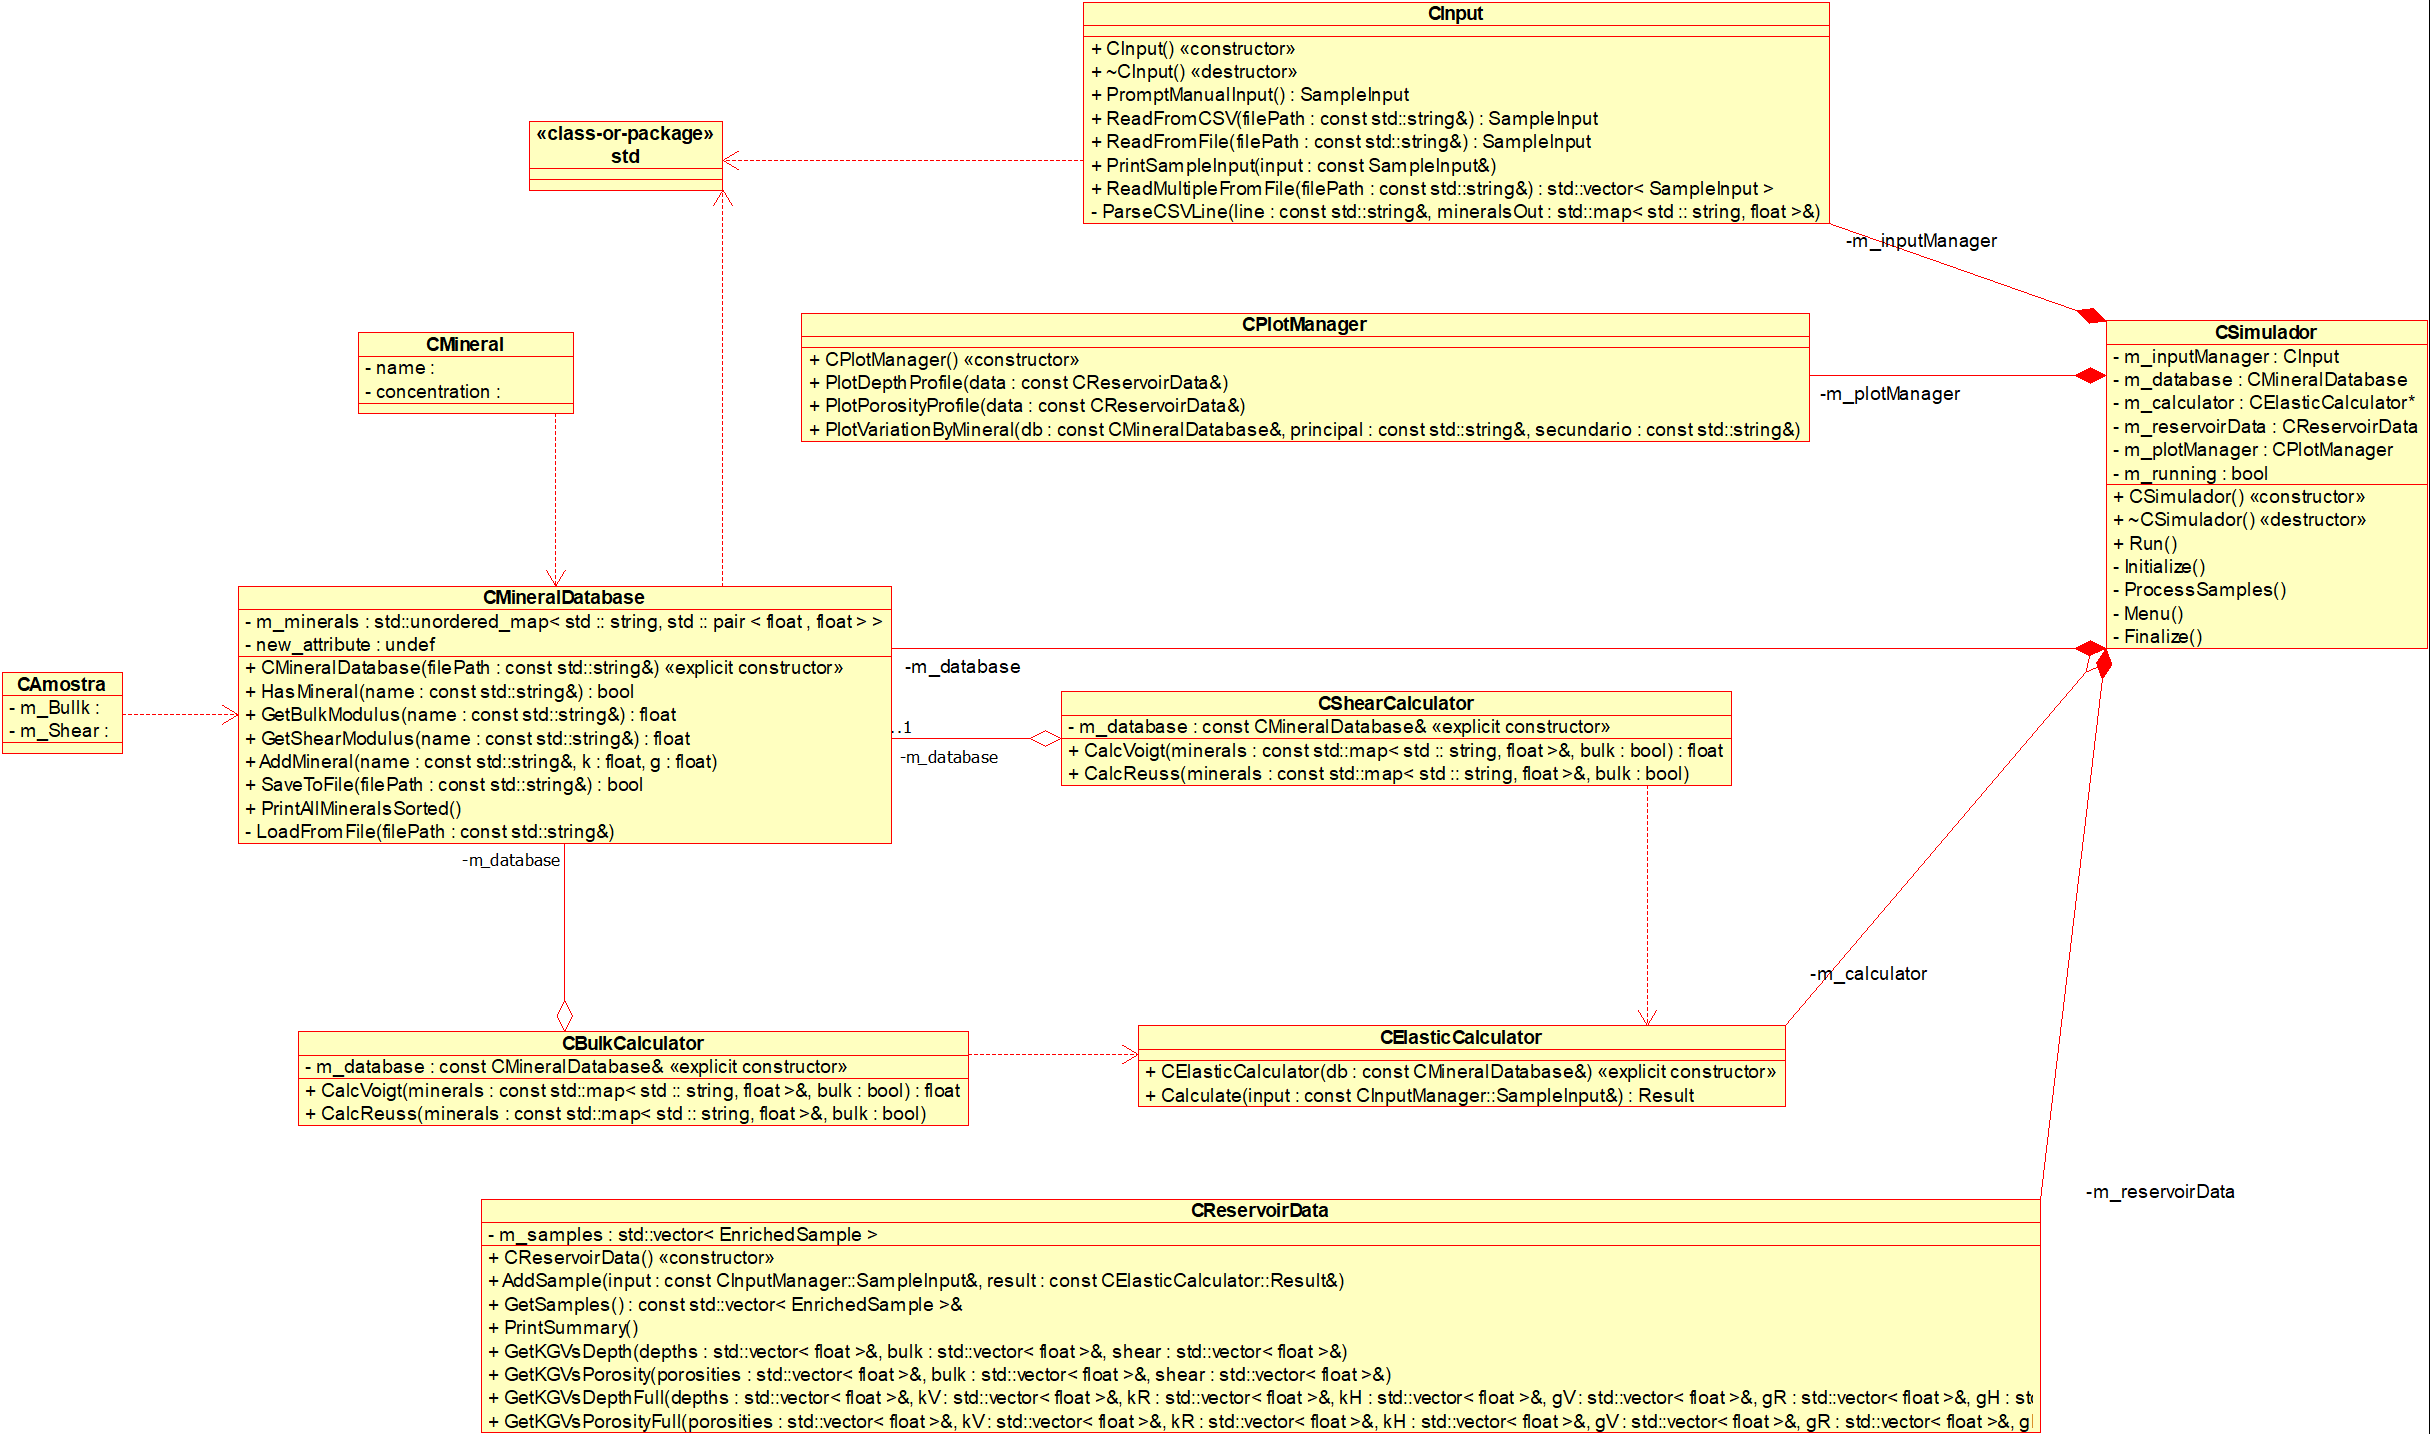
\includegraphics[width=1.0\textwidth]{imagens/Classes.png }
\par\end{centering}
\caption{Diagrama de classes\label{cap:Diagrama-de-classes}}
\end{figure}


\subsection{Dicionário de classes\label{subsec:Dicion=0000E1rio-de-classes}}

\begin{itemize}
    \item \textbf{CSimulator}
    \begin{description}
        \item[Responsabilidade:] Classe principal que orquestra a execução do programa. É responsável por inicializar todos os componentes, gerenciar o menu de interação com o usuário e controlar o fluxo de dados entre os módulos de entrada, cálculo e visualização.
        
        \item[Atributos:] 
        \begin{itemize}
            \item \texttt{-m\_input}: \texttt{CInput} – Instância do gerenciador de entrada de dados.
            \item \texttt{-m\_database}: \texttt{CMineralDatabase} – Instância do banco de dados de minerais.
            \item \texttt{-m\_calculator}: \texttt{CElasticCalculator} – Instância do módulo de cálculo de propriedades elásticas.
            \item \texttt{-m\_reservoirData}: \texttt{CReservoirData} – Instância do repositório de dados das amostras processadas.
            \item \texttt{-m\_plotManager}: \texttt{CPlotManager} – Instância do gerenciador de visualização gráfica.
        \end{itemize}
        
        \item[Métodos:]
        \begin{itemize}
            \item \texttt{+CSimulator() / +\~CSimulator()}: Construtor e destrutor da classe.
            \item \texttt{+Run()}: Inicia e gerencia o laço de execução principal da aplicação.
            \item \texttt{-Initialize()}: Prepara e aloca os recursos para os módulos do sistema.
            \item \texttt{-Menu()}: Exibe as opções disponíveis e captura a escolha do usuário.
            \item \texttt{-ProcessSamples()}: Dispara o fluxo de processamento para uma nova amostra.
            \item \texttt{-Finalize()}: Libera os recursos alocados antes de encerrar a aplicação.
        \end{itemize}
    \end{description}

    \item \textbf{CInput}
    \begin{description}
        \item[Responsabilidade:] Gerencia a aquisição de dados das amostras, seja por meio de entrada manual do usuário no console ou pela leitura e interpretação de arquivos de dados formatados.
        
        \item[Métodos:]
        \begin{itemize}
            \item \texttt{+CInput() / +\~CInput()}: Construtor e destrutor da classe.
            \item \texttt{+PromptManualInput()}: Solicita interativamente os dados da amostra ao usuário.
            \item \texttt{+ReadFromCSV()}: Lê dados de um arquivo no formato CSV (não utilizado na versão final).
            \item \texttt{+ReadFromFile()}: Lê os dados de uma única amostra de um arquivo de texto.
            \item \texttt{+PrintSampleInput()}: Exibe os dados de entrada de uma amostra no console para verificação.
            \item \texttt{+ReadMultipleFromFile()}: Lê uma ou mais amostras de um arquivo de texto.
            \item \texttt{-ParseCSVLine()}: Interpreta uma única linha de um arquivo de dados para extrair a composição mineralógica.
        \end{itemize}
    \end{description}

    \item \textbf{CMineralDatabase}
    \begin{description}
        \item[Responsabilidade:] Encapsula o acesso à base de dados de minerais. É responsável por carregar, salvar e fornecer as propriedades elásticas (módulo de compressibilidade e de cisalhamento) de cada mineral.
        
        \item[Atributos:]
        \begin{itemize}
            \item \texttt{-m\_minerals}: Estrutura de dados que armazena as propriedades dos minerais carregados em memória.
            \item \texttt{-m\_databaseFilePath}: Caminho para o arquivo físico da base de dados.
        \end{itemize}
        
        \item[Métodos:]
        \begin{itemize}
            \item \texttt{+CMineralDatabase(filePath)}: Construtor que inicializa o objeto e carrega os dados do arquivo especificado.
            \item \texttt{+HasMineral(name)}: Verifica a existência de um mineral na base de dados.
            \item \texttt{+GetBulkModulus(name)}: Retorna o módulo de compressibilidade (K) de um mineral.
            \item \texttt{+GetShearModulus(name)}: Retorna o módulo de cisalhamento (G) de um mineral.
            \item \texttt{+AddMineral(name, k, g)}: Adiciona um novo mineral à base de dados em memória.
            \item \texttt{+SaveToFile(filePath)}: Salva o estado atual da base de dados em um arquivo.
            \item \texttt{+PrintAllMineralsSorted()}: Exibe todos os minerais da base de dados em ordem alfabética.
            \item \texttt{-LoadFromFile(filePath)}: Lógica interna para ler e interpretar o arquivo da base de dados.
        \end{itemize}
    \end{description}

    \item \textbf{CElasticCalculator}
    \begin{description}
        \item[Responsabilidade:] Constitui o núcleo de cálculo do sistema. Implementa os modelos de homogeneização de Voigt e Reuss para estimar os módulos elásticos efetivos da matriz rochosa.
        
        \item[Atributos:]
        \begin{itemize}
            \item \texttt{-m\_database}: \texttt{CMineralDatabase\&} – Referência para a base de dados de minerais, utilizada para consultar as propriedades durante o cálculo.
        \end{itemize}
        
        \item[Métodos:]
        \begin{itemize}
            \item \texttt{+CElasticCalculator(db)}: Construtor que recebe uma referência ao banco de dados de minerais.
            \item \texttt{+Calculate(input)}: Orquestra o cálculo para uma amostra, invocando os métodos de Voigt e Reuss e retornando os resultados.
            \item \texttt{-CalcVoigt(minerals, bulk)}: Implementa a média de Voigt para o módulo de compressibilidade ou de cisalhamento.
            \item \texttt{-CalcReuss(minerals, bulk)}: Implementa a média de Reuss para o módulo de compressibilidade ou de cisalhamento.
        \end{itemize}
    \end{description}

    \item \textbf{CReservoirData}
    \begin{description}
        \item[Responsabilidade:] Atua como um repositório para as amostras processadas. Armazena os dados de entrada junto com os resultados calculados para uso posterior em relatórios e gráficos.
        
        \item[Atributos:]
        \begin{itemize}
            \item \texttt{-m\_samples}: Vetor que armazena o conjunto de todas as amostras processadas durante a sessão.
        \end{itemize}
        
        \item[Métodos:]
        \begin{itemize}
            \item \texttt{+CReservoirData()}: Construtor da classe.
            \item \texttt{+AddSample(input, result)}: Adiciona uma nova amostra e seus resultados calculados ao repositório.
            \item \texttt{+GetSamples()}: Retorna uma referência para o vetor completo de amostras.
            \item \texttt{+PrintSummary()}: Exibe no console um resumo com os principais resultados de todas as amostras.
            \item \texttt{+GetKGVvsDepth()}: Extrai e organiza os dados para plotagem de propriedades vs. profundidade.
            \item \texttt{+GetKGVvsPorosity()}: Extrai e organiza os dados para plotagem de propriedades vs. porosidade.
            \item \texttt{+GetKGVvsDepthFull()}: Retorna todos os limites (Voigt, Reuss, Hill) para os perfis de profundidade.
            \item \texttt{+GetKGVvsPorosityFull()}: Retorna todos os limites (Voigt, Reuss, Hill) para os perfis de porosidade.
        \end{itemize}
    \end{description}

    \item \textbf{CPlotManager}
    \begin{description}
        \item[Responsabilidade:] Módulo dedicado à visualização de dados. Utiliza os resultados consolidados em \texttt{CReservoirData} para gerar e exibir gráficos, facilitando a análise e interpretação dos resultados.
        
        \item[Métodos:]
        \begin{itemize}
            \item \texttt{+CPlotManager()}: Construtor da classe.
            \item \texttt{+PlotDepthProfile(data)}: Gera o gráfico dos módulos elásticos em função da profundidade para as amostras fornecidas.
            \item \texttt{+PlotPorosityProfile(data)}: Gera o gráfico dos módulos elásticos em função da porosidade.
            \item \texttt{+PlotVariationByMineral(db, ...)}: Cria gráficos de sensibilidade à variação percentual entre dois minerais.
        \end{itemize}
    \end{description}

\item \textbf{CAmostra}
    \begin{description}
        \item[Responsabilidade:] Encapsula todos os dados pertinentes a uma única amostra de rocha. Funciona como uma estrutura de dados para transportar informações sobre a amostra através do sistema.
        
        \item[Atributos:] 
        \begin{itemize}
            \item \texttt{-m\_reservatorio}: Armazena o nome do reservatório de onde a amostra foi extraída.
            \item \texttt{-m\_nome}: Identificador único da amostra.
            \item \texttt{-m\_profundidade}: Profundidade (em metros) na qual a amostra foi coletada.
            \item \texttt{-m\_porosidade}: Valor percentual da porosidade da rocha.
            \item \texttt{-m\_minerais}: Estrutura de dados (ex.: mapa) que associa o nome de cada mineral à sua proporção na amostra.
        \end{itemize}
        
        \item[Métodos:]
        \begin{itemize}
            \item \texttt{+CAmostra(...)}: Construtor que inicializa todos os atributos do objeto.
            \item \texttt{+NomeReservatorio()}: Retorna o nome do reservatório.
            \item \texttt{+NomeAmostra()}: Retorna o nome da amostra.
            \item \texttt{+Profundidade()}: Retorna o valor da profundidade.
            \item \texttt{+Porosidade()}: Retorna o valor da porosidade.
            \item \texttt{+Minerais()}: Retorna a coleção de minerais e suas respectivas proporções.
        \end{itemize}
    \end{description}

    \item \textbf{CMineral}
    \begin{description}
        \item[Responsabilidade:] Representa a entidade de um mineral, contendo suas propriedades elásticas fundamentais.
        
        \item[Atributos:] 
        \begin{itemize}
            \item \texttt{-m\_name}: O nome do mineral (ex.: Quartzo, Albita).
            \item \texttt{-m\_bulkModulus}: Módulo de compressibilidade (K) do mineral, em GPa.
            \item \texttt{-m\_shearModulus}: Módulo de cisalhamento (G) do mineral, em GPa.
        \end{itemize}
        
        \item[Métodos:]
        \begin{itemize}
            \item \texttt{+CMineral(name, k, g)}: Construtor que inicializa o objeto com os dados do mineral.
            \item \texttt{+Name()}: Retorna o nome do mineral.
            \item \texttt{+BulkModulus()}: Retorna o módulo de compressibilidade (K).
            \item \texttt{+ShearModulus()}: Retorna o módulo de cisalhamento (G).
        \end{itemize}
    \end{description}

    \item \textbf{CShearCalculator}
    \begin{description}
        \item[Responsabilidade:] Especializada no cálculo do módulo de cisalhamento (G) efetivo de uma amostra de rocha, com base em sua composição mineralógica.
        
        \item[Atributos:] 
        \begin{itemize}
            \item \texttt{-m\_db}: Referência à \texttt{CMineralDatabase}, utilizada para consultar propriedades de cisalhamento dos minerais individuais.
        \end{itemize}
        
        \item[Métodos:]
        \begin{itemize}
            \item \texttt{+CShearCalculator(db)}: Construtor que recebe a base de dados de minerais.
            \item \texttt{+CalculateVoigt(amostra)}: Calcula o módulo de cisalhamento efetivo utilizando a média de Voigt (limite superior).
            \item \texttt{+CalculateReuss(amostra)}: Calcula o módulo de cisalhamento efetivo utilizando a média de Reuss (limite inferior).
            \item \texttt{+CalculateHill(amostra)}: Calcula o módulo de cisalhamento efetivo utilizando a média de Hill (média entre Voigt e Reuss).
        \end{itemize}
    \end{description}

    \item \textbf{CBulkCalculator}
    \begin{description}
        \item[Responsabilidade:] Especializada no cálculo do módulo de compressibilidade (K) efetivo de uma amostra de rocha, com base em sua composição mineralógica.
        
        \item[Atributos:] 
        \begin{itemize}
            \item \texttt{-m\_db}: Referência à \texttt{CMineralDatabase}, utilizada para consultar propriedades de compressibilidade dos minerais individuais.
        \end{itemize}
        
        \item[Métodos:]
        \begin{itemize}
            \item \texttt{+CBulkCalculator(db)}: Construtor que recebe a base de dados de minerais.
            \item \texttt{+CalculateVoigt(amostra)}: Calcula o módulo de compressibilidade efetivo utilizando a média de Voigt.
            \item \texttt{+CalculateReuss(amostra)}: Calcula o módulo de compressibilidade efetivo utilizando a média de Reuss.
            \item \texttt{+CalculateHill(amostra)}: Calcula o módulo de compressibilidade efetivo utilizando a média de Hill.
        \end{itemize}
    \end{description}
    
\end{itemize}




\section{Diagrama de seqüência -- eventos\index{Eventos} e mensagens\index{Mensagens}\index{Diagrama de sequência}\label{subsec:diagrama de sequ=0000EAncia}}


\subsection{\textit{\emph{Diagrama de sequência geral\label{subsec: Diagrama de sequ=0000EAncia geral}}}}

Veja o \textit{\emph{diagrama de seqüência na}} Figura \ref{cap:Diagrama-de-sequencia}.

\begin{figure}[H]
\begin{centering}
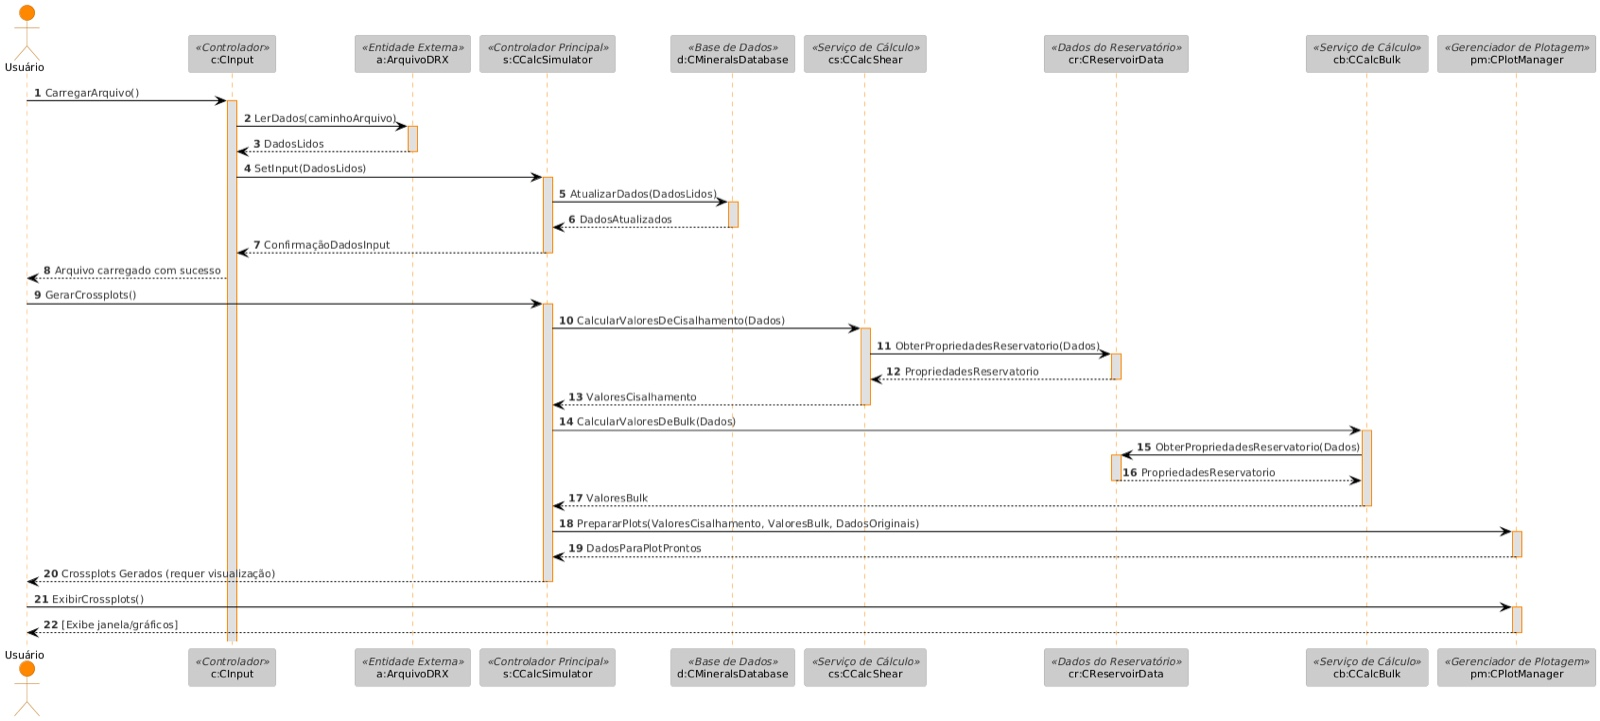
\includegraphics[width=1\textwidth]{imagens/SequenciaGeral.jpeg}
\par\end{centering}
\caption{Diagrama de seqüência geral\label{cap:Diagrama-de-sequencia}}
\end{figure}


\subsection{\textit{\emph{Diagrama de sequência específico\label{subsec: Diagrama de sequ=0000EAncia espec=0000EDfico}}}}

\begin{figure}[H]
\begin{centering}
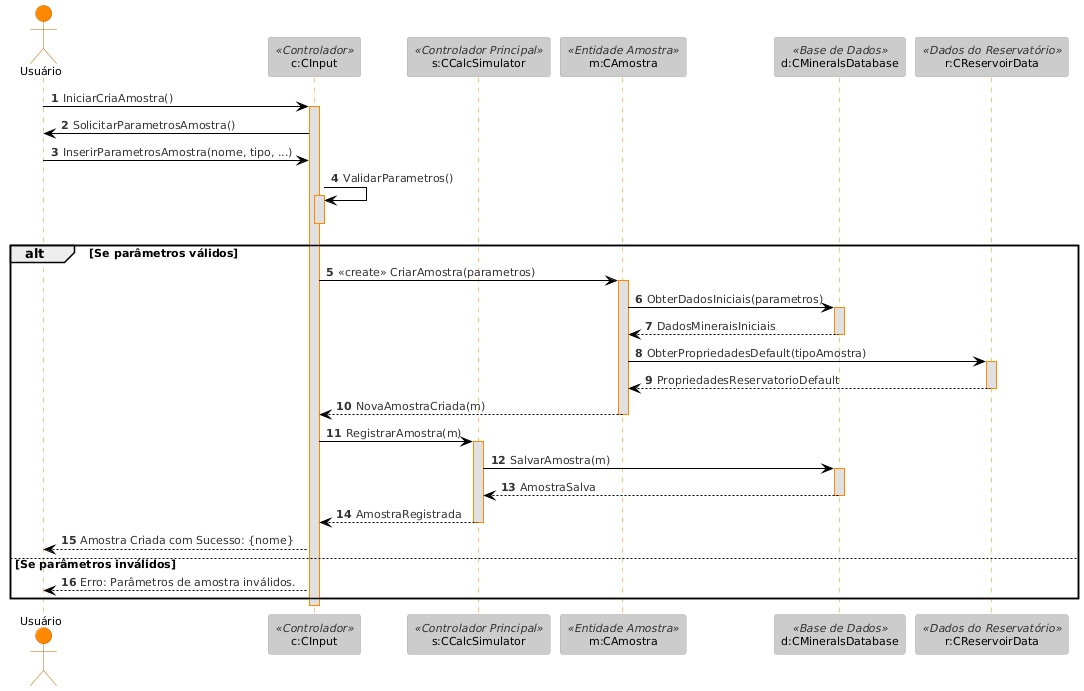
\includegraphics[width=1\textwidth]{imagens/SequenciaEspecifico.jpeg}
\par\end{centering}
\caption{Diagrama de seqüência específico\label{cap:Diagrama-de-sequencia-especifico}}
\end{figure}


\section{Diagrama de comunicação\index{comunicação} -- colaboração\index{colaboração}\label{subsec:Diagrama-de-Comunica=0000E7=0000E3o}\index{Diagrama de colaboração}\label{par:Diagrama-de-colabora=0000E7=0000E3o:} }

No diagrama de comunicação o foco é a interação e a troca de mensagens
e dados entre os objetos. 

Veja na Figura \ref{subsec:Diagrama-de-Comunica=0000E7=0000E3o} o
diagrama de comunicação mostrando a sequência de interação, onde a aplicação solicita leitura do arquivo da amostra para dar prosseguimento com o cálculo das propriedades, onde busca os dados do banco de dados. A aplicação armazena os dados e gera os resultados, e por fim solicita a geração dos gráficos de perfil.

\begin{figure}[H]
\begin{centering}
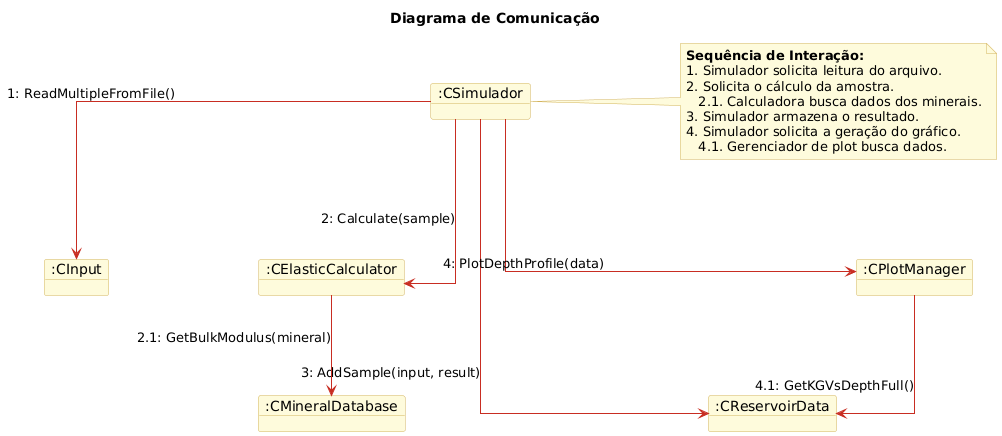
\includegraphics[width=1\textwidth]{imagens/Comunicacao.png}
\par\end{centering}
\caption{Diagrama de comunicação\label{cap:Diagrama-de-comunica=0000E7=0000E3o}}
\end{figure}


\section{Diagrama de estado\index{estado}\index{Diagrama de estado}\label{subsec:diagrama de estados}}


Veja na Figura \ref{cap:Diagrama-de-maquina-de-estado} o diagrama
de máquina de estado para o objeto CSimulador

\begin{figure}[H]
\begin{centering}
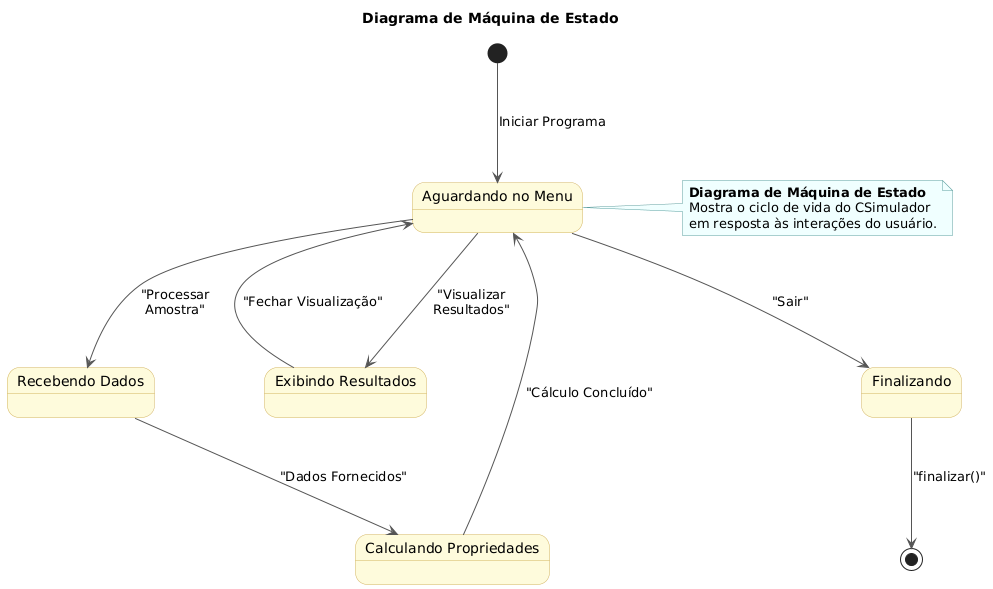
\includegraphics[width=1\textwidth]{imagens/MaquinaDeEstado.png}
\par\end{centering}
\caption{Diagrama de máquina de estado\label{cap:Diagrama-de-maquina-de-estado}}
\end{figure}


\section{Diagrama de atividades\label{sec: Diagrama de atividades}}

w

Veja na Figura \ref{cap:Diagrama-de-atividades} o diagrama de atividades. 

O processo se inicia no Nó Inicial, levando diretamente à primeira Atividade, que é "Apresentar Menu Principal". Neste ponto, uma decisão importante é oferecida ao usuário: se a opção for "Sair", o fluxo é desviado diretamente para a finalização do programa; caso contrário, ao escolher "Processar Amostra", o sistema avança para uma segunda decisão que define o método de entrada dos dados, seja através da atividade "Carregar de Arquivo" ou da criação manual. Uma vez que os dados da amostra são fornecidos por um desses caminhos, o fluxo converge e prossegue de forma sequencial para a fase de processamento, onde a atividade central de "Executar cálculos de propriedades poroelásticas" é realizada.

Com o término dos cálculos, indicado pelo estado "Resultados calculados e disponíveis", uma nova decisão permite ao usuário escolher entre "Gerar Gráficos" ou "Mostrar Relatórios" para a análise final. Concluída esta etapa, o diagrama chega ao seu ciclo de execução principal, onde a última decisão do fluxo pergunta se o usuário "Deseja realizar outra operação?". Uma resposta afirmativa reinicia todo o processo, retornando o controle ao menu principal para um novo ciclo de trabalho. Caso a resposta seja negativa, o fluxo segue para a atividade "Finalizar Software" e culmina no Nó Final, que representa o encerramento completo da aplicação.

\begin{figure}[H]
\begin{centering}
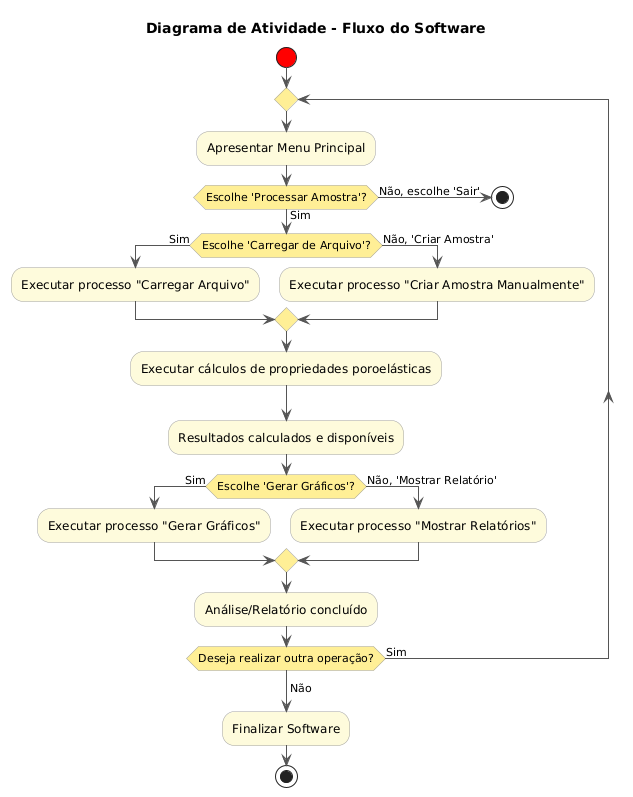
\includegraphics[width=1\textwidth]{imagens/Atividade-FluxoDoSoftware.png}
\par\end{centering}
\caption{Diagrama de atividades\label{cap:Diagrama-de-atividades}}
\end{figure}


